\documentclass[a4paper,11pt]{article}
\usepackage[utf8]{inputenc}
\usepackage{graphicx}
\usepackage{amsmath}
\usepackage[a4paper, left=3cm, right=3cm, top=3cm, bottom=2cm]{geometry}
\usepackage{enumitem}
\usepackage{minted}
\usepackage{xcolor}
\usepackage{booktabs}
\usepackage{caption}

% Pour les parties de codes
\usepackage{listings}
\lstset{
    basicstyle=\ttfamily\small,
    keywordstyle=\color{blue}\bfseries
}


\begin{document}

\title{Détection et Classification de Panneaux de Signalisation Routière}
\author{Demessance Victor, Kozdeba Mathieu}
\date{UTC - SY32 - P2024}
\maketitle

\renewcommand{\contentsname}{}
\tableofcontents

\newpage

\section{Introduction}
De nombreuses recherches sont menées sur la reconnaissance d'objets. Dans des contextes routiers, c'est un défi d'importance majeur que de pouvoir détecter et reconnaitre des informations capitales telles que la signalisation. Aujourd'hui, la plupart des véhicules sont équipés de systèmes d'assistance de conduite (ADAS). Par exemple, les images des panneaux de signalisation sont captées par une caméra fixée à l'avant du véhicule. \textbf{L'objectif de ce projet est de construire un processus de détection et de reconnaissance d'informations de signalisation routière (hors temps réel). L'idée sera d'utiliser des méthodes d'apprentissage supervisé classiques ainsi que des réseaux de neurones convolutifs.}

\vspace{2mm}

\noindent Les différentes données utilisées ont pu être récoltées et labellisées par les étudiants suivant l'UV \textbf{SY32} à l'UTC. 

\vspace{2mm}

\noindent Les différents labels de notre étude sont : 
\begin{itemize}[noitemsep]
\item danger
\item interdiction
\item obligation
\item stop
\item ceder
\item frouge
\item forange
\item fvert
\item \textit{empty (une classe permettant de rajouter la nuance des négatifs pour nos classifieurs)}
\end{itemize}

\section{Analyse exploratoire}

\subsection{Chargement des données}

Afin d'assurer le chargement des données, nous avons pu créer une fonction de \textbf{parsing} et \textbf{linkage} des répertoires d'images et de labels. L'objectif est d'obtenir un dictionnaire contenant toutes les informations pour notre étude, sous la forme : 

\begin{minted}[frame=single, linenos, fontsize=\footnotesize]{python}
{
    "Key (=XXXX)": {      # Indice of the image/label (pk)
        "img" :           # image as an array,
        "labels" : {
            "Indice" : {  # Indice of the label (pk auto-increment)
                "name" :  # name of the label,
                "coord" : # [xmin, ymin, xmax, ymax],
                "img" :   # cropped img of the label
            }
        }
    }
}
\end{minted}

Il nous est par la suite possible de traiter ces données en les convertissant relativement rapidement en des tableaux X et Y \textit{(pour de l'apprentissage supervisé)} ou en Dataset \textit{(torch.utils.data.Dataset())} selon le besoin.

\vspace{2mm}

Afin d'accélérer le processus de chargement/déchargement des données et d'éviter l'importation depuis les répertoires en un dictionnaire à chaque nouveau processus, il a également été utilisé lors du développement un système de sérialisation depuis le module json de python. En utilisant json, il devient très simple de sauvegarder nos données de manière structurée dans un fichier ainsi que de les charger dans d'autres scripts Python.

\subsection{Critique du dataset}

Dans l'idée de proposer une étude des plus précise, il peut sembler pertinent de juger la qualité de nos données.  Ce dataset d'images et de labels a été créé par les étudiants de SY32. Ainsi, la quantité d'images disponibles pour chaque label n'est pas énorme. Elle ne permet pas d'entraîner correctement les classifieurs sans éviter des biais de poids sur les modèles. De plus, il y a environ 100 images de chaque panneau mais seulement 50 pour chaque type de feu. Ce nombre est très faible et la détection de feux soulèvera plus de problèmes que celle des panneaux. Certaines images ont aussi une qualité discutable, ce qui peut amoindrir la qualité des caractéristiques visuelles extraites. Enfin, les éléments à détecter peuvent faire la taille entière de l'image ou n'être juste qu'une petite zone de l'image, ce qui peut compliquer la détection et l'entraînement du modèle d'apprentissage.

\section{Apprentissage supervisé}

\subsection{Méthodologie}

La méthodologie appliquée afin de mettre en place un système de détection et de classification de panneaux est la suivante :

\begin{enumerate}[label=\arabic*.]
    \item \textbf{Analyser les données labellisées} afin d'\textbf{extraire les caractéristiques visuelles} les plus pertinentes.
    \item \textbf{Construire une stratégie de classification} efficace à l'aide d'un ou plusieurs classifieurs (binaires ou multiclasse).
    \item Mettre en place une \textbf{démarche de proposition de fenêtres} (recherche sélective, fenêtre glissante...) pour initier le processus de détection.
    \item \textbf{Classifier les fenêtres détectées} et \textbf{harmoniser} les résultats (seuillage par probabilité de prédiction, filtrage...).
    \item \textbf{Extraire les faux positifs} et \textbf{ré-entraîner le modèle} de classification afin d'améliorer ses performances.
\end{enumerate}

\subsection{Caractéristiques visuelles}

Avant de débuter le travail de classification, il est nécessaire de posséder des caractéristiques visuelles performantes et pertinentes pour convertir nos images avant leur traitement. Pour cela, plusieurs stratégies ont été mises en pratique. 

\vspace{2mm}

Tout d'abord, nous avons recherché des caractéristiques visuelles pertinentes pour classifier nos données. En premier lieu, les histogrammes de gradient (HOG) témoigne d'une réelle mine d'informations utiles à donner à nos classifieurs.

\begin{figure}[H]
    \centering
    \includegraphics[width=12cm]{HOG_example.png}
    \caption{Exemple d'application des HOG sur une image}
    \label{fig:enter-label}
\end{figure}

\noindent Pour rappel, les HOG sont des descripteurs de forme basés sur l'orientation des gradients locaux dans une image \textit{(Figure n°1)}. Ils sont basés sur l'hypothèse que la forme d'un objet peut être approximée par la distribution locale des directions des gradients ou des contours de l'image.

\vspace{2mm}

\noindent Par ailleurs, les informations de couleur nous ont semblé très rapidement être des données capitales à extraire lors de la classification de signalisation routière. La différence de couleur est en effet un moyen efficace de différencier les panneaux ronds interdiction et obligations mais aussi les trois couleurs de feu. De plus, les couleurs des signalisations ont tendance à se démarquer du reste de l'image.

L'information de couleur doit donc être ajoutée aux données HOG de l'image. Pour la récupérer, nous utilisons l'image sous sa forme HSV.

\noindent Le HSV est un espace en 3D permettant de définir une couleur selon 3 critères : 

\begin{itemize}[noitemsep]
    \item \textbf{Teinte (Hue)} : Représente la teinte de la couleur en elle même.
    \item \textbf{Saturation} : Indique la pureté de la couleur, de 0\% à 100\%.
    \item \textbf{Valeur} : Désigne la luminosité de la couleur, de 0 (noir) à 100\% (blanc).
\end{itemize}

\begin{figure}[H]
    \centering
    \includegraphics[width=6cm]{HSV_example.png}
    \caption{Définition du modèle HSV (teinte, saturation, valeur}
    \label{fig:enter-label}
\end{figure}

\noindent Après différents tests, il se trouve que seule la teinte (Hue) est utile lors de la classification. Afin d'éviter la surdimensionalité et le poids du modèle, nous allons donc seulement garder cette information. Une image sera donc traduite en un vecteur contenant des données HOG et HSV (seulement le Hue ).

\vspace{4mm}

\subsection{Méthodes de classification}

\subsubsection{Classification multiclasse}

La première méthode de classification, que l'on pourra qualifier de "brute", fut d'appliquer directement notre classifieur sur les données vectorisées dans un problème de classification multiclasse. 

\vspace{2mm}

\noindent L'annexe n°1 nous renseigne sur les résultats de cette méthode. On peut facilement apercevoir que les performances augmentent bien avec l'utilisation des caractéristiques définies dans la section précédente. 

\noindent Les conclusions suivantes peuvent être tirées :

\begin{itemize}[noitemsep]
    \item Le classifieur \textbf{Knn} montre des performances relativement bonnes lors de l'utilisation des HOG et de la teinte. \textit{Le nombre de voisins 8 a été choisi après quelques tests.}
    \item Le classifieur \textbf{SVM} affiche des taux d'erreurs relativement bas sur toutes les configurations, nous avons choisi le noyau polynomial qui donnait les meilleurs résultats.\textbf{ Il est donc l'outil de choix à sélectionner pour classifier nos images.}
    \item \textbf{Decision Tree} montre une amélioration en passant de 41.1\% (image brute) à 28.8\% (HOG + Hue). Malgré tout, il reste l'un des classifieurs les moins performants.
    \item Pour le classifieur \textbf{Random Forest}, les résultats restent correctes entre les différentes configurations sans pour autant être très intéressants. \textit{Le paramètre n=100 est celui par défaut et semble être le meilleur.}
    \item \textbf{AdaBoost} présente une mauvaise performance générale, ne permettant pas de faire mieux qu'un classifieur aléatoire pour cette tâche et/ou avec ces caractéristiques. Nous avons testé différentes valeurs de n et n=10 restait celui avec les meilleurs résultats en moyenne.
\end{itemize}



\subsubsection{Classification binaire}

Afin de perfectionner le modèle, nous avons pu réfléchir à différentes pistes d'amélioration. L'un des problèmes majeurs est dans la diversité des classes que nous avons à difféncier. L'une des solutions peut être de diviser ce problème afin d'augmenter les performances de chaque problème de décision. 

\vspace{2mm}

\noindent La première de nos idées fut de créer 2 classifieurs multiclasses regroupant d'un côté les panneaux et de l'autres les feux. En effet, ces 2 instances étant très différentes, il nous a semblé pertinent de les séparer pour les traiter. 
Après analyse, nous avons pu conclure que l'idée de diviser pour mieux performer était la bonne direction. Cependant, la qualité des résultats pourrait être bien meilleure si nous divisions encore plus notre problème. Pour cela, nous avons donc créé un classifieur binaire par label. Ainsi, l'entrainement des classifieurs se fait sur le même dataset, avec 1 pour la classe en question et une valeur négative pour tous les autres labels \textit{(ainsi que 3 images aléatoires négatives par image vide, ce qui équilibre la distribution de classe "empty")}.

\vspace{2mm}

\noindent Les résultats sont visibles en Annexe n°2. Les paramètres sont identiques à la classification multiclasse. Cependant, les performances sont ici drastiquement meilleures. On approxime même des taux d'erreur de 0\% dans certaines classes, ce qui confronte notre étude au nombre de données de validation disponible. En effet, cette valeur n'a aucun sens statistique si ce n'est l'expression d'une valeur très faible d'erreur dû au fait qu'il n'y avait pas assez d'images à tester.

\subsubsection{Classification binaire \& multiclasse}

Une autre stratégie testée fut de regrouper les labels des différents feux afin de simplifier la reconnaissance de ceux-ci en augmentant la taille des données positives. En effet, nous ne disposons pas de beaucoup de photos de feu, ce qui biaise les classifieurs. Regrouper les feux en un unique label dans un nouveau classifieur multiclasse, puis reprendre la classification binaire permettant de déterminer quelle est la couleur du feu est une technique efficace pour augmenter nos performances.


\subsubsection{Conclusion}

La stratégie de classification adoptée consiste à entraîner un classifieur de type SVM avec un noyau polynomial pour chaque label étudié. Dans le cas des feux, on classifie les feux en général puis le type de feu en second ordre.

\vspace{2mm}

\noindent A propos de la taille de nos images, il a fallu réfléchir à une taille vers lesquelles les redimensionner avant de les classifier. Après des ajouts au fichier d'analyse statistique du dataset, on sait qu'un label a une taille moyenne d'environ \textbf{119x138} pixels. Après plusieurs tests, il se trouve que les dimensions \textbf{100x100} semblent être un bon compromis entre quantité d'informations et besoins de calcul.

\subsection{Fenêtre de détection}
La phase de détection est la partie la plus complexe du projet. Il faut tout d'abord analyser l'image pour potentiellement trouver un objet puis ensuite le classifier à l'aide des classifieurs préalablement entraînés sur notre dataset. Les méthodes de détection sont décrites ci-dessous:

\subsubsection{Fenêtres glissantes}

La méthode de détection par \textbf{fenêtre glissante} consiste à faire glisser sur l'image en cours de traitement une fenêtre de taille fixe. Cependant, nous nous sommes rapidement rendu compte que cela serait très peu efficace étant donné la diversité des images fournies. En effet, les panneaux peuvent avoir différentes tailles et angles de prise de vue, il nous est donc nécessaire d'adapter notre fonctionnalité de fenêtre glissante. 

\vspace{2mm}

\noindent La première de notre amélioration a été de passer à la méthode des \textbf{fenêtres glissantes dynamiques}. Celle-ci consiste aussi à faire glisser une fenêtre sur l'image mais cette fois, le processus est répété avec plusieurs tailles de fenêtres.

\vspace{2mm}

\noindent La seconde, permettant d'améliorer les performances de classification des feux de signalisation tout en répondant aux contraintes d'entrées des classifieurs, fut de mettre en place \textbf{deux fenêtres glissantes successives}. Pour cela, on s'est intéressé aux ratios de taille de nos différents labels. Pour les panneaux, ce ratio (largeur/hauteur) est de \textbf{1.009}, on utilisera ainsi un carré comme fenêtre. Pour les feux de signalisation, ce ratio est de \textbf{0.434}, le format de la fenêtre sera donc différent afin de proposer aux classifieurs des images au plus proche de ce qu'ils ont pu avoir en entrainement.

\vspace{2mm}

\noindent L'un des principaux problèmes de cette méthode est le temps de calcul demandé. En effet, pour chaque fenêtre, il faut extraire les caractéristiques visuelles, puis lancer la prédiction de chaque classifieur et enfin supprimer les doublons. Ainsi avec cette méthode, nous mettions environ une heure pour parcourir la totalité du dataset val.

\subsubsection{Recherche Selective}

\textbf{La recherche selective} est un algorithme permettant de proposer des fenêtres candidates suite à une segmentation de l'image. Cette méthode se trouve être assez chronophage et complexe à développer "\textit{from scratch}". Cependant, la librairie d'opencv propose une implémentation rapide de ce mécanisme. Afin de l'utiliser, on combine son implémentation avec un seuil d'aire minimum de fenêtre. Pour obtenir ce seuil, on effectue des statistiques sur toutes nos données d'entrainement. Le \textit{quantile(0.05) (=300px²)}, assurant une perte de moins de \textit{5\%} des panneaux (\textit{qui de toute manière n'aurait pas eu de grande chances d'être classifié correctement de part leurs tailles}), permet déja de réduire de moitié les propositions négatives de fenêtres candidates. Lors de l'utilisation de cette algorithme, les performances de la détection augmentent drastiquement de par l'absence d'un grand nombre de faux positifs (\textit{du aux multiples filtres des candidats proposés aux classifieurs}). Cependant, nous avons augmenté l'aire minimale requise au fur et à mesure de nos test et nous avons atteint la valeur de 3500 px² empiriquement. Cette valeur ne permet pas de détecter les plus petits panneaux mais a permis de diminuer grandement le nombre de faux positifs. C'est la solution finale que nous avons retenu.

\vspace{2mm}

\noindent En plus de la condition sur l'aire de la fenêtre détectée, nous avons ajouté des conditions sur la forme de la fenêtre. En effet, nous avons remarqué que de nombreuses fenêtres étaient des rectangles "allongés", c'est à dire que la largeur ou la hauteur du rectangle étaient disproportionnées par rapport à l'autre. Ainsi les fenêtres ayant une largeur supérieure à 1,5 fois la hauteur et une hauteur supérieure à 3,5 fois la largeur ne sont pas étudiées. Ces valeurs ont été déterminés empiriquement. Nous avons affiné cette condition pour les panneaux en réduisant la hauteur possible a 1,5 fois la largeur mais aussi pour les feux avec une hauteur supérieure à 1,5 fois la largeur. Ainsi, la fenêtre contenant un panneau doit ressembler à un carré et celle du rectangle à un rectangle en hauteur. Toutes ces conditions réduisent grandement le temps de calcul nécessaire et les faux positifs.

\subsection{Détection et classification} 

\subsubsection{Classification des fenêtres candidates}

Une fois les fenêtres candidates proposées à nos classifieurs, nous traitons cela par 2 processus distincts. Pour les panneaux, les classifieurs binaires jouent leur rôles indépendamment les uns des autres. Pour les feux, notre classifieur général indique la présence d'un feu, puis c'est aux 3 classifieurs binaires de couleurs de feu de renvoyer le type de feu détecté.

\subsubsection{Filtrage et suppression de fenêtres classifiées}
 
Tous nos classifieurs ont été créés avec la configuration de sortie de probabilité (plutot que sortir une valeur de classe). Ainsi, il nous est possible d'effectuer un premier filtre sur les données de classification. Pour les panneaux, (les classifieurs étant binaires, la classe de sortie possède au moins 0.5 de probabilité) nous posons un seuil à \textbf{0.7} de score. Pour les feux, nous posons à \textbf{0.9} le seuil du premier classifieur de détection de feu. En effet, ce classifieur étant plus général, nous avons pu remarquer que le nombre de faux positifs était bien plus grand. De plus, les scores des vrais positifs étaient plus élevés. Enfin, pour les couleurs des feux, les seuils sont fixés à \textbf{0.7} comme pour les panneaux.

\vspace{2mm}

\noindent Par la suite, nous appliquons un algorithme de \textbf{Non Maximum Suppression} avec seuil d'\textbf{IoU} (Intersection on union) à \textbf{0.1}. Ce seuil est un paramètre que nous avons fait évoluer au cours de nos analyses. Il s'est révélé être le plus performant. En effet, les panneaux ne se chevauchent que rarement, il n'est donc pas réellement risqué de poser ce genre de seuil si bas.

\subsection{Gestion des résultats}

Compte tenue de la définition de nos classifieurs, il nous a été nécessaire d'effectuer plusieurs méthodes afin de réentrainer tous les classifieurs. En effet, les feux de signalisation sont d'abord détectés par un classifieur binaire, avant d'être soumis à une nouvelle classification sur leur couleur. La gestion des résultats s'est donc passée en 2 étapes afin de ne pas rater de classifieur.

\begin{enumerate}[label=\arabic*.]
    \item Obtention des résultats de la classification binaire des feux (toutes couleurs confondues) de label "feux" et réentrainement des classifieurs avec les faux positifs
    \item Une fois que le classifieur de détection des feux généraux est optimal, on effectue le réentrainement sur les labels finaux "fvert", "forange", "frouge".
\end{enumerate}

\subsubsection{Entrainement des faux positifs}

L'entrainement des faux positifs s'est fait avec 2 stratégies différentes. La première fut de seulement prendre comme détecteur de faux positifs un filtre calculant les valeurs d'IoU entre les bounding box labélisées prédites et celles réelles. Dans ce cas, les valeurs de classes n'influent en rien et l'on ne traitera donc pas les erreurs de classification (par exemple un panneau étant détecté positif par le classifieur de feux.). 

\noindent L'autre stratégie fut de traiter à la fois l'IoU et la classe prédite. Ainsi, l'on peut définir comme faux positif une bounding box se placant sur un panneau réel, mais étant de la mauvaise classe. 

\vspace{2mm}

\noindent \textit{La seconde stratégie nous a semblé plus pertinente et plus efficace dans notre cas, puisqu'elle simule au mieux ce qu'aurait donné un algorithme de détection de faux positifs sur le classifieur multiclasse de notre problème de base. C'est donc elle que nous avons gardé.}

\vspace{2mm}

A la suite de l'entrainement sur les faux positifs, nous obtenons un taux de précision très élevé au détriment d'un rappel de qualité. Les éléments à détecter deviennent bien plus difficiles à extraire, surement du à un déséquilibre factuel de répartition des classes sur le réentrainement (bien trop de négatifs, ce qui biaise les classifieurs)...

\subsubsection{Résultats}

\textit{Ces résultats se réfèrent aux Annexe n°4 à 8.}

\vspace{2mm}

\noindent On peut remarquer que l'AP sans classification est assez similaire entre les datasets VAL et TEST avec près de 70\% des objets détectés, cependant seuls environ 55\% des objets sont correctement classifiés. Cependant, on peut observer une différence de près de 10\% pour le rappel entre les datasets VAL et TEST et que celui a une valeur plutôt faible ce qui indique que notre programme possède encore beaucoup de faux positifs.

\vspace{2mm}

\noindent Concernant chaque label pris un à un, nous obtenons les résultats suivants :

\begin{itemize}[noitemsep]
    \item \textbf{Danger :} Le classifieur possède une précision assez élevée mais il y a beaucoup d'oublis.
    \item \textbf{Interdiction :} Le classifieur est plus efficace sur le dataset VAL que sur le dataset TEST. Cela peut être du à la petite quantité de données d'entrainement, ce qui baisse la capacité de généralisation.
    \item \textbf{Obligation} : Le classifieur obligation est plus précis sur les données VAL que sur les TEST mais le rappel est identique. 
    \item \textbf{Stop :} Le classifieur stop reste le plus efficace avec une précision de 1 et un rappel assez haut.
    \item \textbf{Ceder :} Le classifieur ceder obtient également de bonnes performances quelque soit le jeu de données.
    \item \textbf{Feux (frouge, forange, fvert):} Pour ces trois classifieurs, la précision est très basse sur les données VAL et le rappel est également très faible. Les courbes fvert et frouge sont absentes du graphique TEST ce qui indique qu'aucun n'a été correctement détecté. 
\end{itemize}


\section{Apprentissage Profond}

\subsection{Méthodologie}

La méthodologie employée pour l'apprentissage par réseau de neurone fut de proposer un réseau d'extraction des caractéristiques visuelles et de classification des fenêtres candidates.

\noindent Pour obtenir ces propositions de fenêtres, nous avons mis en place une méthode de recherche sélective sur nos images afin d'en ressortir des candidats à classifier. Par la suite, nous procédons à une extraction des caractéristiques de notre image via couches de convolutions. Enfin, le réseau classifie les données obtenues dans le cadre d'un problème multiclasse. 

\subsection{Architecture du réseau SignNet}

A la suite d'un processus de recherche sélective, les fenêtres passent dans un réseau de neurone que l'on nommera \textbf{\textit{SignNet}}.

\vspace{2mm}

\noindent Les paramètres de notre réseau ont pu être testés récursivement de manière à les perfectionner au mieux. Ceux choisis sont les suivant :

\begin{table}[h!]
    \centering
    \begin{tabular}{|c|c|c|}
        \hline
        \textbf{Nombre d'epochs} & \textbf{Taille d'un batch} &\textbf{Taille des images d'entrées} \\
        \hline
        30 & 20 & 3x64x64\\
        \hline
    \end{tabular}
\end{table}

La première piste de travail vu d'appliquer directement ce réseau de classification sur les fenêtres issues de la recherche sélective. De cette manière, les performances de classification sont de 95\% environ (Visible en Annexe n°9). Cependant, lors de la détection (\textit{malgré l'utilisation de filtres de surface et de NMS}), les performances d'un tel classifieur ne sont pas du tout optimales. Il a donc été nécessaire de revoir notre architecture (Annexe n°8) pour s'approcher de celle d'un réseau R-CNN.

\vspace{2mm}

Pour cela, on ajoute une méthode à SignNet de manière a ne le faire qu'extraire les caractéristiques visuelles de l'image d'entrée. Par la suite, on associe ces images avec le label et l'on entraine un classifieur SVM à définir un modèle d'apprentissage sur ces données. Après différents test, le noyau polynomial semble être le plus performant.

\vspace{2mm}

\noindent Malheureusement, les résultats obtenues à la suite de cette méthode ne sont pas assez bons. Le réseau ne semble pas extraire des caractéristiques visuelles assez spécifique pour classifier le panneau/feu de signalisation. Cela peut s'expliquer par différents facteurs tels que la taille de redimensionnement de nos images, la stratégie de fenêtrage, l'architecture du réseau de neurones. 

\subsubsection{Résultats}

Pour conclure sur la partie d'apprentissage profond, il ne nous est pas possible de proposer des données de résultats utilisables pour évaluer nos performances. Notre étude s'arrête à la création d'un classifieur performant (95\% de taux de succès), mais ayant de fortes lacunes dans la phase de détection. Malgré nos tentatives de modification des paramètres, tel que l'équilibrage du nombre de panneaux d'interdictions (par sur/sous échantillonage), la création de plus d'échantillons aléatoires négatifs, la modification des paramètres du réseau (taux d'apprentissage, nombre d'epochs, taille du batch), nous n'avons pas pu améliorer ces performances. 

\section{Conclusion}
\subsection{Problèmes rencontrés}
Ce projet a permis de développer un système de détection et de classification de panneaux de signalisation routière en utilisant à la fois des méthodes classiques et des techniques d'apprentissage profond. Les résultats montrent que le projet peut encore être amélioré car il reste quelques problèmes.

\vspace{2mm}

\noindent Le premier est le temps d'exécution du programme. En effet, une image met entre 5 et 20 secondes à être traîtée par le programme d'apprentissage supervisé. Ce temps est beaucoup trop long pour qu'il soit utilisable sur une voiture autonome par exemple. C'est donc un point sensible sur lequel il est possible d'imaginer des optimisations. 

\vspace{2mm}

\noindent Le deuxième est la qualité de détection et de classification du programme. Nous avons toujours beaucoup de faux positifs et oublis de panneaux. Ces faux positifs et oublis sont parfois compréhensibles du fait de la qualité de l'image traîtée ou de l'état réel du panneau (couleurs effacées, panneau déformé, panneau recouvert...) et d'autres fois nous ne savons pas ce qui perturbe le classifieur. Nous ressentons particulièrement ce problème avec les feux qui sont extrêmement mal détectés et classifiés.

\subsection{Pistes d'amélioration}

La première amélioration pouvant être apportée au projet est un meilleur dataset. En effet, nous pensons qu'il n'y avait pas assez d'images d'entraînement pour les classifieurs et qu'en même temps, celles-ci étaient trop diversifiées. C'est à dire que les panneaux font parfois la taille de l'image et d'autres fois moins de 3000 pixels carrés, les angles de prises de vue sont aussi parfois très différents. Pour autant, le dataset pourrait être réutilisé par la prochaine promotion de SY32 qui y ajouterait leurs images. Ainsi, au fil des années, le dataset gagnerait en qualité.

\vspace{2mm}

\noindent Concernant le temps de traîtement des images, nous n'avons pas vraiment d'idées sur la façon de régler ce problème. Nous savons que la méthode des fenêtres glissantes est rapidement chronophage, mais la recherche sélective l'est aussi, ainsi changer de méthode de détection pourrait peut-être diminuer le temps de traîtement. Nous ne savons pas si le fait d'avoir de multiples classifieurs binaires à la place d'un seul classifieur multiclasse augmente ce temps ou non. 

\newpage
\section{Annexes}

\captionsetup[table]{labelformat=simple, labelsep=colon, name=Annexe, justification=centering}


\begin{table}[H]
\centering
\begin{tabular}{lccc}
\toprule
\textbf{Classifieur} & \textbf{Image brute} & \textbf{HOG} & \textbf{HOG + Hue} \\
\midrule
Knn(8) & 31.1 & 17.9 & 12.3 \\
SVM SVC(poly) & 11.6 & 9.1 & 8.8 \\
Decision Tree & 41.1 & 38.6 & 28.8 \\
Random Forest(100) & 15.1 & 16.6 & 15.5 \\
AdaBoost(10) & 52.9 & 52.7 & 48.1 \\
\bottomrule
\end{tabular}
\caption{Taux d'erreur en \% des classifieurs multiclasses en fonction des caractéristiques utilisées}
\label{tab:classification-results}
\end{table}

\begin{table}[H]
\centering
\small % Réduction de la taille de la police
\setlength{\tabcolsep}{3pt} % Réduction de l'espace entre les colonnes
\begin{tabular}{@{}lcccccccr@{}}
\toprule
\textbf{Classifieur} & \textbf{Danger} & \textbf{Interdiction} & \textbf{Obligation} & \textbf{Stop} & \textbf{Ceder} & \textbf{Frouge} & \textbf{Forange} & \textbf{Fvert} \\
\midrule
Knn & 0 & 6.0 & 0.7 & 0 & 0.7 & 0.6 & 4.0 & 1.3 \\
SVM & 0 & 2.1 & 0.7 & 0 & 0 & 6.4 & 2.8 & 0 \\
Random Forest & 0.7 & 7.9 & 7.3 & 0.7 & 0.7 & 8.6 & 4.0 & 1.3 \\
AdaBoost & 0 & 4.6 & 2.6 & 0 & 0.7 & 4.0 & 2.6 & 1.3 \\
\bottomrule
\end{tabular}
\caption{Taux d'erreur en \% des classifieurs binaires pour chaque labels}
\label{tab:classification-results}
\end{table}
\textit {Ces résultats restent indicatifs mais ne sont pas forcément fixes. C'est-à-dire que lorsque les classifieurs sont réentrainés, nous n'obtenons pas forcément les résultats des tableaux mais des valeurs proches.}


\begin{table}[H]
\centering
\begin{tabular}{lccc}
\toprule
\textbf{AP (sans classif)} & \textbf{AR (sans classif)} & \textbf{mAP (avec classif)} & \textbf{mAR (avec classif)} \\
\midrule
67.58 & 32.27 & 54.67 & 36.55 \\
\bottomrule
\end{tabular}
\caption{Résultats évaluation sur VAL}
\end{table}

\begin{table}[H]
\centering
\begin{tabular}{lccc}
\toprule
\textbf{AP (sans classif)} & \textbf{AR (sans classif)} & \textbf{mAP (avec classif)} & \textbf{mAR (avec classif)} \\
\midrule
70.07 & 23.53 & 55.29 & 28.61 \\
\bottomrule
\end{tabular}
\caption{Résultats évaluation sur TEST}
\end{table}

\begin{table}[H]
    \centering
    \includegraphics[width=10cm]{mkozdeba_2024_06_23_13_56_51_829113.png}
    \caption{Courbe de précision/rappel des résultats sur le dataset VAL}
    \label{fig:enter-label}
\end{table}

\begin{table}[H]
    \centering
    \includegraphics[width=10cm]{mkozdeba_2024_06_23_14_16_15_174773.png}
    \caption{Courbe de précision/rappel des résultats sur le dataset TEST}
    \label{fig:enter-label}
\end{table}

\begin{table}[H]
    \centering
    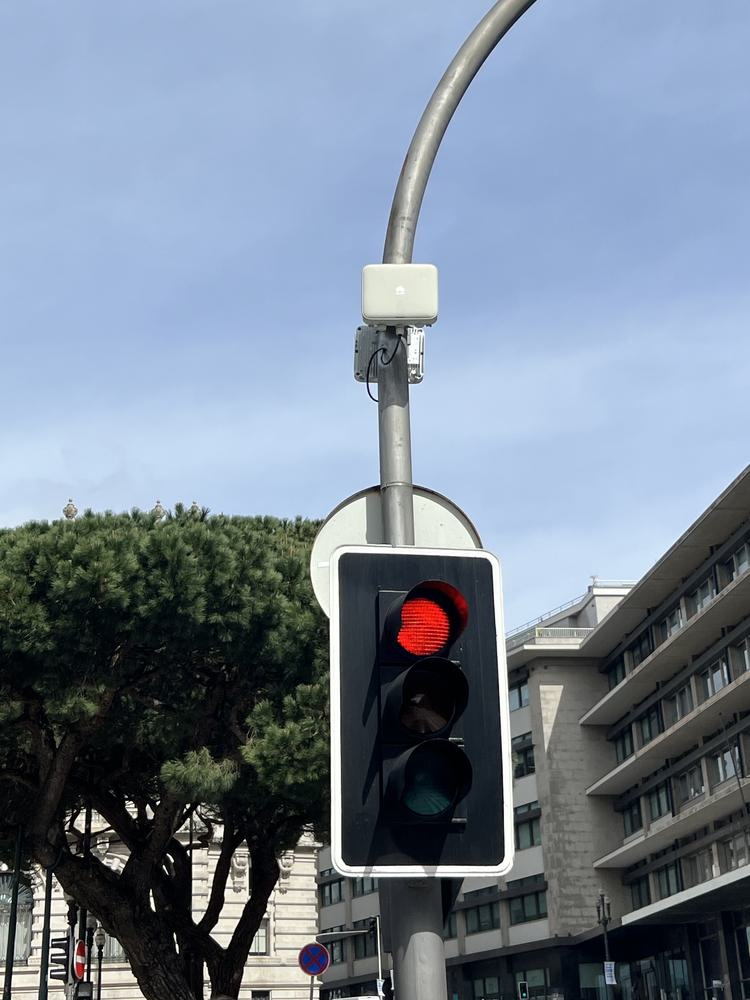
\includegraphics[width=4cm]{0004.png}
    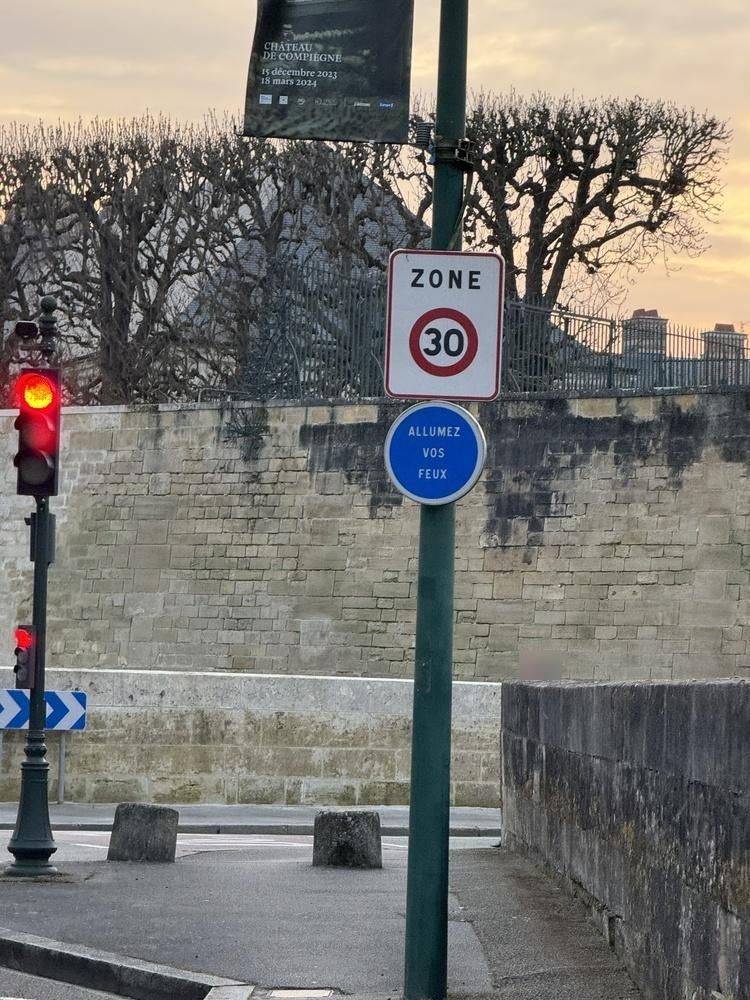
\includegraphics[width=4cm]{0054.png}
    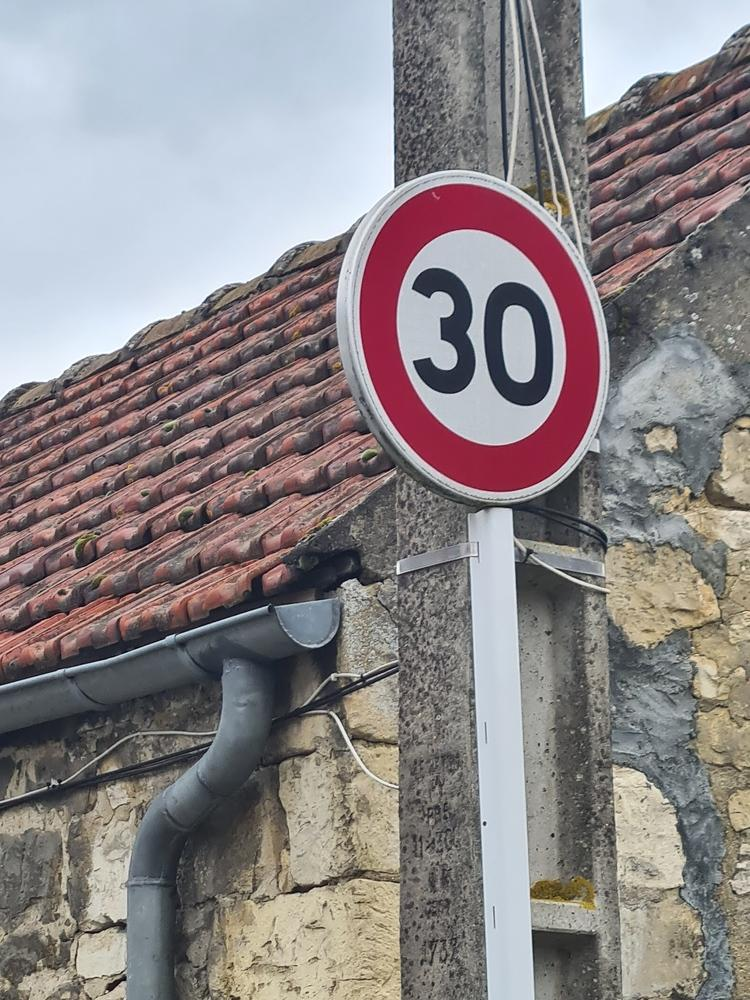
\includegraphics[width=4cm]{0083.png}
    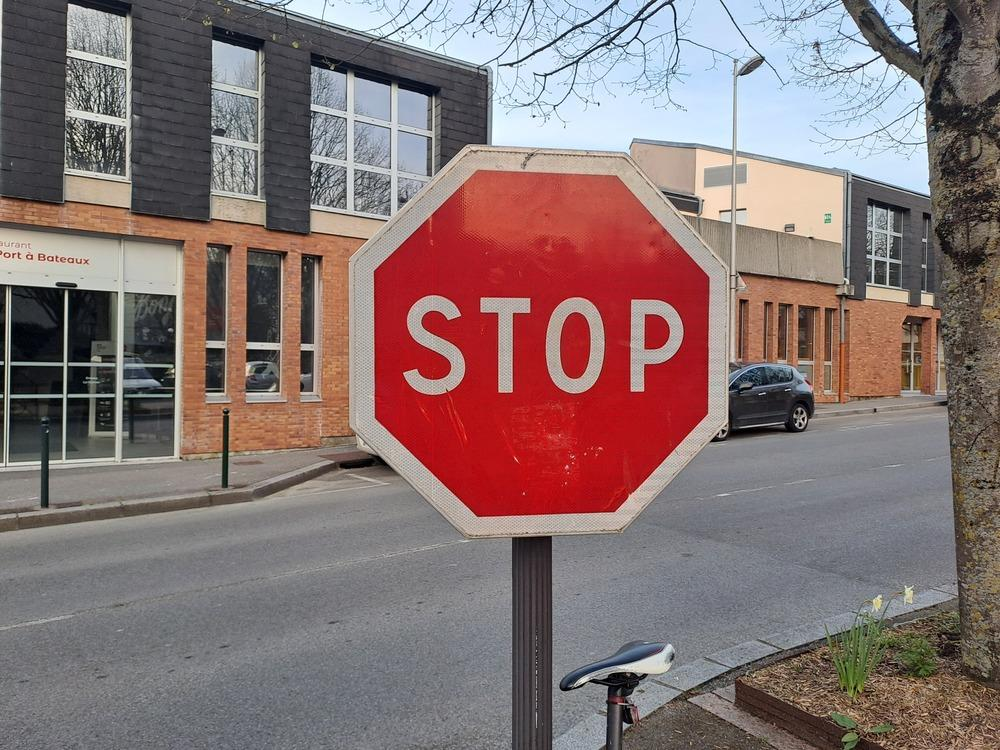
\includegraphics[width=4cm]{0088.png}
    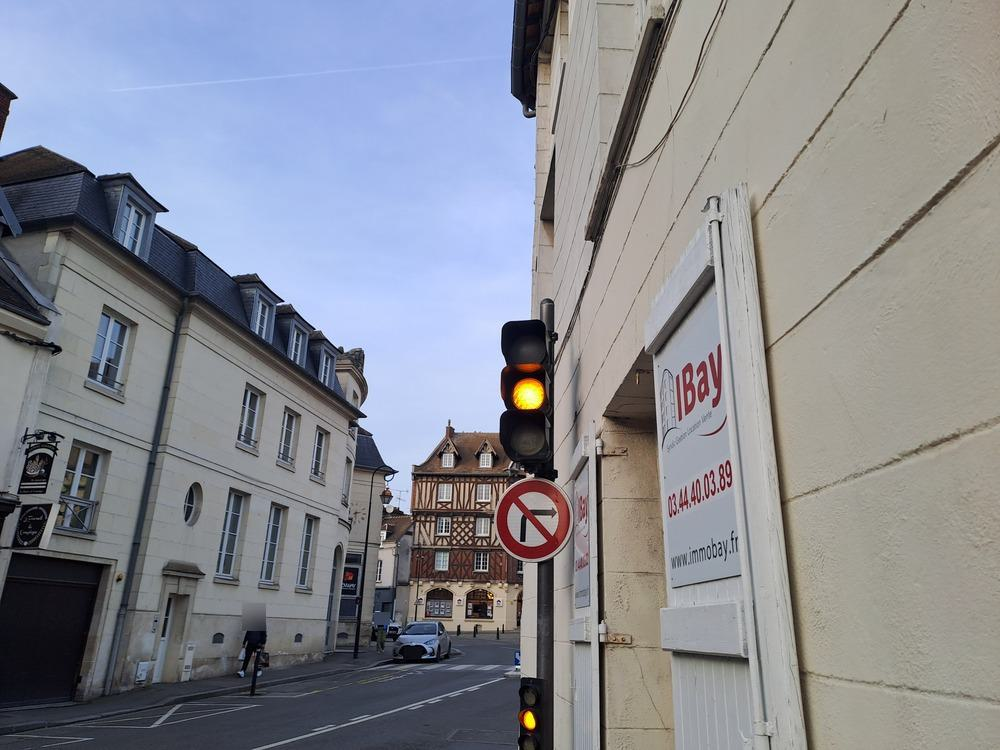
\includegraphics[width=4cm]{0137.png}
    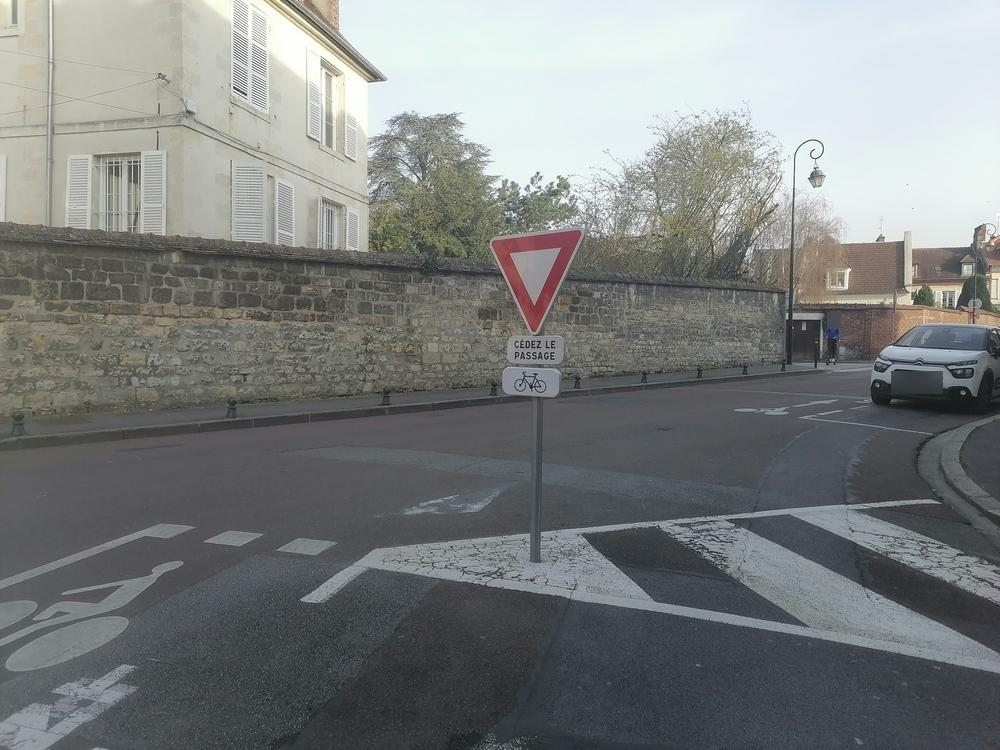
\includegraphics[width=4cm]{0240.png}
    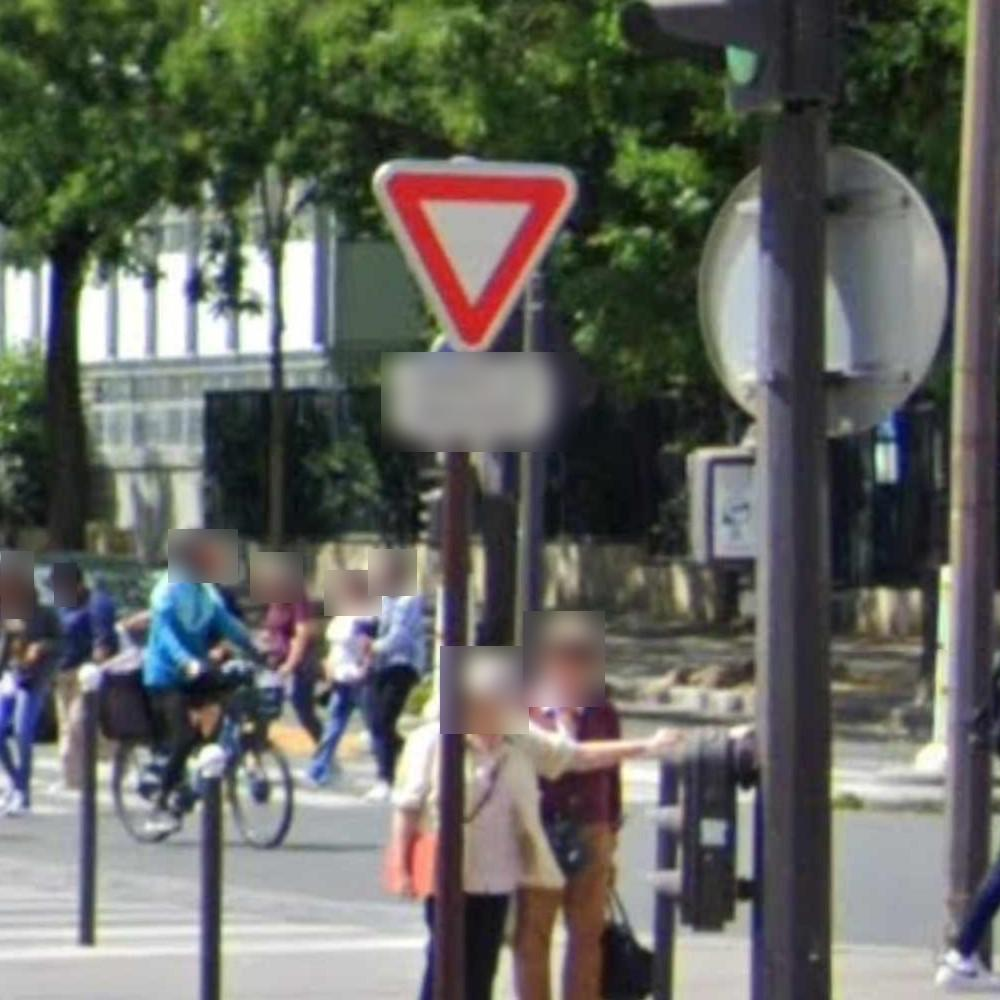
\includegraphics[width=4cm]{0263.png}
    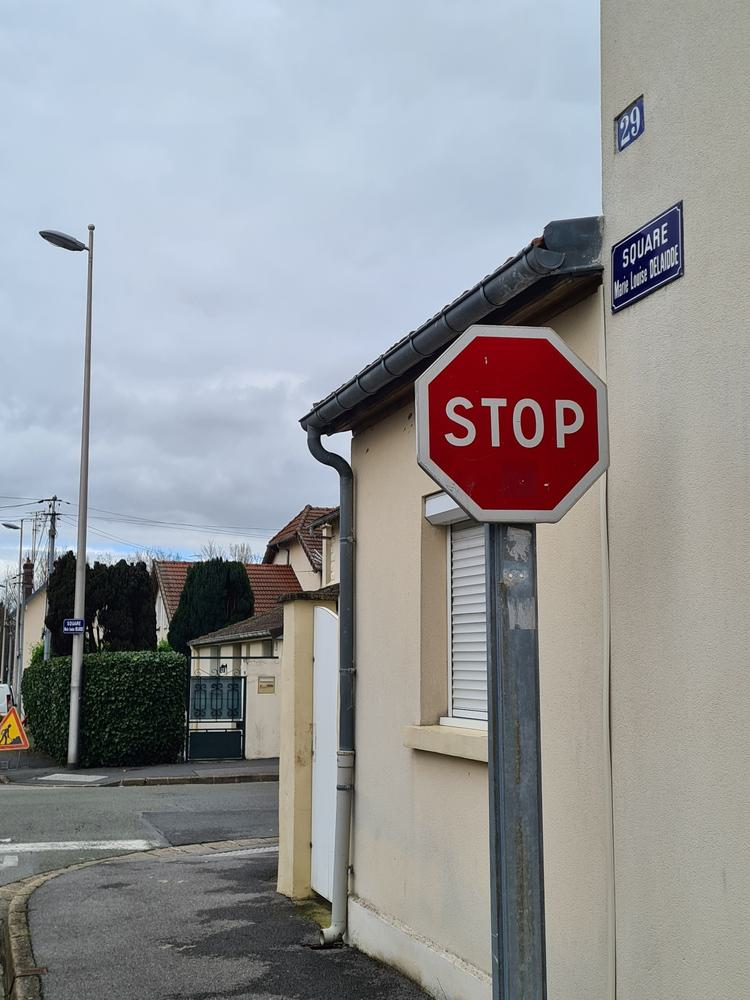
\includegraphics[width=4cm]{0272.png}
    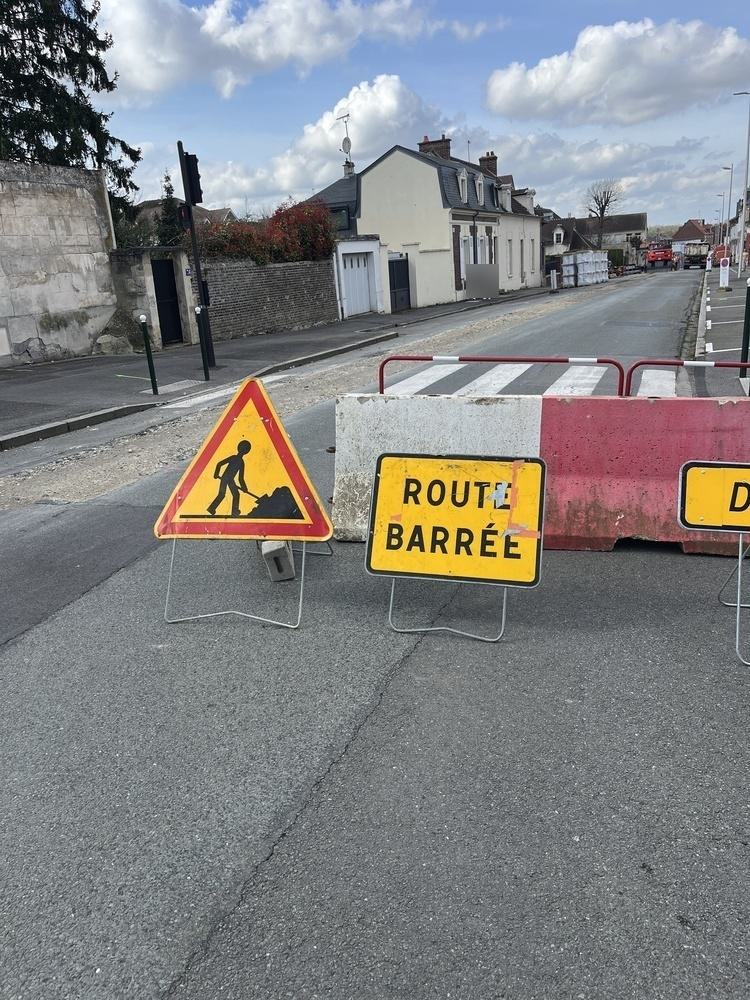
\includegraphics[width=4cm]{0343.png}
    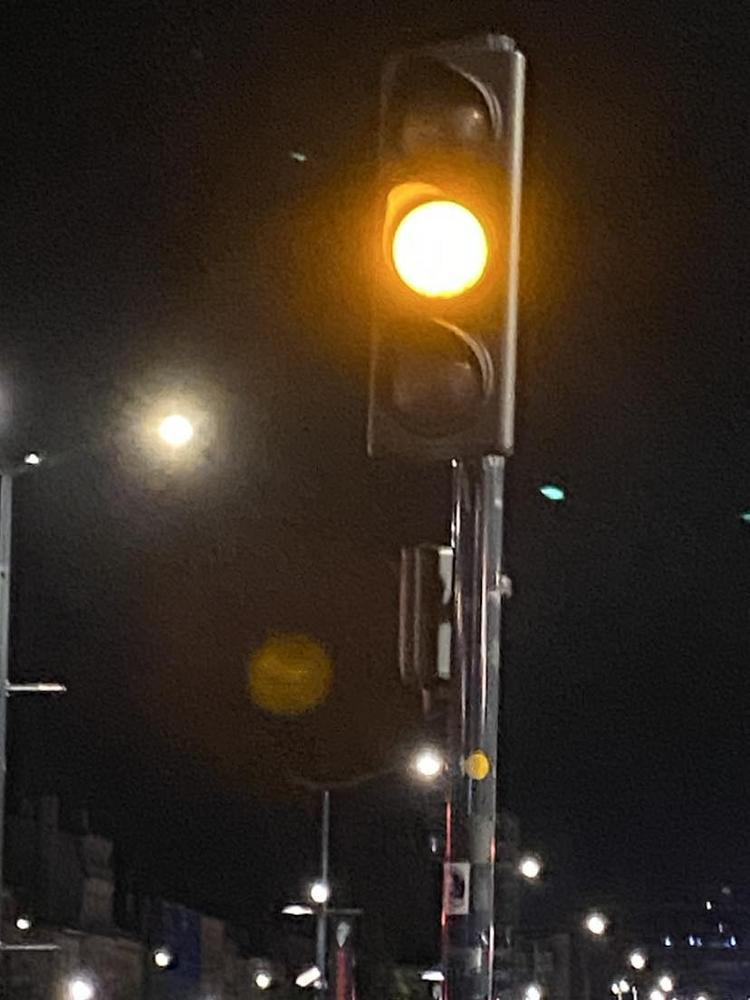
\includegraphics[width=4cm]{0358.png}
    \caption{Résultats divers de l'apprentissage supervisé sur VAL}
    \label{fig:enter-label}
\end{table}

\begin{table}
 \begin{tabular}{|c|c|c|c|c|}
    \hline
    \textbf{Layer (type)} & \textbf{Input Shape} & \textbf{Output Shape} & \textbf{Number of Parameters} \\
    \hline
    Conv2d-1 & [3, 64, 64] & [32, 64, 64] & 896 \\
    \hline
    Conv2d-2 & [32, 64, 64] & [32, 64, 64] & 10,144 \\
    \hline
    MaxPool2d-3 & [32, 64, 64] & [32, 32, 32] & 0 \\
    \hline
    Conv2d-4 & [32, 32, 32] & [64, 32, 32] & 28,640 \\
    \hline
    Conv2d-5 & [64, 32, 32] & [64, 32, 32] & 65,568 \\
    \hline
    MaxPool2d-6 & [64, 32, 32] & [64, 16, 16] & 0 \\
    \hline
    Linear-7 & [64*16*16] & [128] & 1,048,704 \\
    \hline
    ReLU-8 & [128] & [128]& 0 \\
    \hline
    Dropout-9 & [128] & [128] & 0 \\
    \hline
    Linear-10 & [128] & [num\_classes] & 1,049,736 \\
    \hline
    \end{tabular}
    \caption{Architecture du réseau SignNet}
\end{table}

\begin{table}[h!]
    \centering
    \begin{tabular}{|c|c|c|}
        \hline
        \textbf{Époque} & \textbf{Perte} & \textbf{Erreur d'entraînement} \\
        \hline
        1  & 0.6130  & 0.5022 \\
        2  & 0.4492  & 0.3430 \\
        3  & 0.0094  & 0.2706 \\
        4  & 0.1576  & 0.2276 \\
        5  & 0.2157  & 0.1968 \\
        6  & 0.0073  & 0.1748 \\
        7  & 0.0069  & 0.1556 \\
        8  & 0.0793  & 0.1399 \\
        9  & 0.0007  & 0.1281 \\
        10 & 0.0334  & 0.1171 \\
        11 & 0.0378  & 0.1078 \\
        12 & 0.0247  & 0.1001 \\
        13 & 0.0296  & 0.0934 \\
        14 & 0.0106  & 0.0873 \\
        15 & 0.0006  & 0.0819 \\
        16 & 0.0002  & 0.0772 \\
        17 & 0.0003  & 0.0730 \\
        18 & 0.0003  & 0.0692 \\
        19 & 0.0000  & 0.0659 \\
        20 & 0.0027  & 0.0630 \\
        \hline
    \end{tabular}
    \caption{Performances du réseau de classification par epochs (méthode 1)}
    \label{tab:performances}
\end{table}

\end{document}
